\chapter{Grundlagen der Implementierung} % (fold)
\label{cha:implementierung_Überblick}

Wie im Kapitel "Design" gefordert, wurde zur Umsetzung des Werkzeugs ein "Tangible Tabletop Interface" verwendet. Tabletop Interface zeichnen sich im Generellen dadurch aus, dass im Gegensatz zu handelsüblichen Rechnern nicht nur die Software sondern auch die Hardware applikationsspezifisch ist und nicht generisch eingesetzt werden kann. Die Hardware bildet dabei einen Teil oder die gesamte Benutzungsschnittstelle ab. Im speziellen Fall eines "Tangible Tabletop Interfaces" basiert der Benutzerinteraktion auf der Verwendung physischer Bausteine ("Tokens"), die auf der physischen Oberfläche des Interfaces manipuliert werden. Dieses Paradigma wird ergänzt von Tabletop Interfaces, die die Benutzerinteraktion ausschließlich auf Gesten bzw. Berührungen der Oberfläche abbilden (horizontal verbaute "Touch-" bzw. "Multi-Touch-Displays").

REFs!!! Die Entwicklung von Tabletop Interfaces begann Mitte der 1990er-Jahren mit den Arbeiten von Ishii \& Ullmer. Auch die erste Anwendung, die sich mit Modellierungs-Ansätzen mit Hilfe von Tabletop Interfaces konzentriert, stammt aus dieser Zeit. Mit dem fortschreiten der technologischen Entwicklung ist heute ein Status erreicht, in dem mit Hilfe generischer Identifikations-Frameworks schnell und ohne großen Aufwand Applikationen mit "tangiblen" Inputkanälen erstellt werden können. Zur Zeit noch im Prototypenstatus befinden sich Ansätze, die sich mit generischen Möglichkeiten des tangiblen Informationsoutputs beschäftigt. Der Rückkanal vom Rechner zum Benutzer wird heute zumeist mit der Projektion von Inhalten auf die Arbeitsoberfläche umgesetzt.

In den folgenden Abschnitten wird die historische Entwicklung von Tabletop Interfaces sowie der aktuelle Stand der Entwicklung im Anwendungsbereich dieser Arbeit betrachtet. Es werden dabei die grundlegenden Konzepte und Eigenschaften der jeweiligen Arbeiten betrachtet und das Potential hinsichtlich der Umsetzung von in Kapitel XY identifizierten Anforderungen an das hier entwickelte Werkzeug betrachtet. 

\section{Historische Entwicklung von Tangible Interfaces} % (fold)
\label{sec:entwicklung_tangible_interfaces}

Erste Arbeiten: \citep{Wellner93a}, \citep{Suzuki95}

Vision für Bildung: \citep{Resnick98}, Manifestation: \citep{Zuckerman05}

Der Begriff der Tangible bzw. Graspable Interfaces – also der "berührbaren" oder "begreifbaren" Benutzungsschnittstellen — stammt aus der Mitte der neunziger Jahre des zwanzigsten Jahrhunderts. \citet{Fitzmaurice95} werden im Allgemeinen als die ersten betrachtet, die den Begriff des "Graspable User Interfaces" prägen und damit die Manipulierbarkeit digitaler Information durch physische Mittel beschreiben. \citet{Fitzmaurice96} präzisiert später den Begriff durch die Abgrenzung zwischen (herkömmlichen, maus-, tastatur- und bildschirmbasierenden) zeitlich gemultiplexten Schnittstellen, bei denen der Informationsaustausch zwischen Benutzer und System über einen Kanal zeitlich hintereinander erfolgt und den (neuartigen, berührbaren) räumlich gemultiplexten Schnittstellen, bei denen mehrere Kanäle gleichzeitig zur Interaktion zwischen Benutzer und System verwendet werden können. 

Der Begriff des "Tangible User Interfaces" (TUI) wurde kurz danach bzw. parallel dazu von \citet{Ishii97} eingeführt. \citeauthor{Ishii97} verfolgen dabei bei der Definition den umgekehrten Weg und sprechen von einer "Augmentation der realen Welt durch eine Kopplung von digitaler Information and physische Objekte"\footnote{\emph{“augment the real physical world by coupling digital information to everyday physical objects and environments”}\citep{Ishii97}}. 

\subsection{Ubiquitous Computing}

\subsection{Augmented Reality} 

\subsection{Metaphern} % (fold)
\label{ssub:metaphern}

% subsubsection metaphern (end)

\subsection{Tangible Output} % (fold)
\label{ssub:tangible_output}

Aktuatoren \citep{Patten07}

% subsubsection tangible_output (end)

% section entwicklung_tangible_interfaces(end)

\section{Konzeptualisierung und Klassifikation von Tangible Interfaces} % (fold)
\label{sec:konzeptualisierungen_von_tangible_interfaces}

Die Entwicklung des Forschungsgebiets der "Tangible Interfaces" wurde von mehreren konzeptuellen Arbeiten maßgeblich beeinflusst. Die dort vorgeschlagenen Erklärungsmodelle definieren das Gebiet und grenzen es gegenüber anderen Forschungsbereichen ab. Sie dienen außerdem als Grundlage für Erklärung und Konzeption konkreter Tangible Interfaces. Im Folgenden wird die historische Entwicklung dieser konzeptuellen Modelle beschrieben und auf deren Spezifika eingegangen.

Zur strukturierten Betrachtung von Tangible Interfaces ist es außerdem notwendig, jene Dimensionen zu identifizieren, an denen sich einzelne Tangible Interfaces einordnen und unterscheiden lassen. Die Ausprägungen dieser Dimensionen liefern kombiniert ein Begriffssystem, dass bei der Aufbereitung von unterschiedlichen Ansätzen im Bereich der Tangible Interface sowie deren Vergleich helfen kann. Die hier vorgestellten Ansätze tragen unterschiedlich detailliert und aus unterschiedlichen Gesichtspunkten zu dieser Thematik bei. Die einzelnen Ansätze werden hier dargestellt und in Kapitel XY auf das in dieser Arbeit entwickelte System angewandt um so das System-Design aus konzeptueller Sicht zu reflektieren und potentielle Verbesserungs- und Erweiterungsmöglichkeiten zu identifizieren.

Allgemein ist anzumerken, dass eine Vielzahl von Ausdrücken im sich entwickelnden Forschungsgebiet mehrfach belegt wurden und/oder nicht eindeutig definiert sind. Im Folgenden werden die Ausdrücke der jeweiligen Autoren übernommen, eine Interpretation bzw. Abbildung auf die Terminologie anderer Autoren wird nur vorgenommen, wo sie im jeweiligen Artikel explizit angeführt wurde. In der Zusammenfassung dieses Abschnitts wird versucht, die unterschiedlichen Terminologien nochmals zusammenzufassen und einen Satz an Ausdrücken festzulegen, der im Folgenden für diese Arbeit Anwendung findet.

Am Ende jeder Beschreibung sind in einer tabellarischen Zusammenfassung jeweils die zentralen Konzepte und Beiträge des Ansatzes angeführt. Die Tabelle weist einheitlich Einträge zu folgenden Themen auf:
\begin{description}
 \item[Kategorien] Kategorien von Tangible Interfaces, die im Beitrag identifiziert werden  (inkl. Unterscheidungsmerkmal zur Kategoriebildung)
 \item[Konzepte] Konzepte, die bei der Betrachtung bzw. beim Design eines Tangible User Interfaces zur Anwendung kommen 
 \item[Eigenschaften] Eigenschaften, die ein Tangible User Interface bzw. dessen Komponenten aufweisen können
 \item[PD-Brücke] Aussagen, die der Beitrag zur Natur oder Ausgestaltung der Brücke zwischen physische und digitaler Welt macht
\end{description}

Wird in einem Beitrag keine Aussage zu einem oder mehreren dieser Themen gemacht, so ist dies explizit durch "---" angeführt.

Die Ansätze, die in dieser Betrachtung berücksichtigt wurden, sind in der Reihenfolge der zeitlichen Entstehung angeordnet. Eine Beschreibung und Visualisierung der kausalen Zusammenhänge und Bezugnahmen erfolgt in der Zusammenfassung der Ergebnisse in Abschnitt \ref{sub:tui_konzepte_zusammenfassung}. Bei der Beschreibung der Arbeiten wird nicht auf sämtliche vorgestellten Aspekte eingegangen, sondern fokussiert jene Teile vorgestellt, die sich mit der Konzeptualisierung oder Klassifikation von Tangible User Interfaces beschäftigen. Die berücksichtigten Ansätze sind im Einzelnen:

%\begin{multicols} {2}
    \begin{itemize}
    	\item Bricks \citep{Fitzmaurice95}
    	\item Graspable User Interfaces \citep{Fitzmaurice96}
    	\item Tangible Bits \citep{Ishii97}
    	\item Containers, Tokens und Tools \citep{Holmquist99}
		\item Tangible Object Meaning \citep{Underkoffler99}
    	\item Das MCRpd Interaktions-Modell \citep{Ullmer00}
    	\item Tokens and Constraints \citep{Ullmer02}
    	\item Degree of Coherence \citep{Koleva03}
    	\item Tokens and Constraints zur Spezifikation \citep{Shaer04}
    	\item Kategorien von \gls{TUI}-Anwendungen \citep{Klemmer04}
    	\item Tangible User Interfaces Taxonomy \citep{Fishkin04}
    	\item Mixed Reality \citep{Coutrix06}
    	\item Tangible Bits: Beyond Pixels \citep{Ishii08}
    \end{itemize}
%\end{multicols}

\subsection{Bricks} % (fold)
\label{sub:bricks}

Mit dem Bricks-System stellen \citet{Fitzmaurice95} das erste als „Graspable User Interface“ bezeichnete System vor. Das in dieser Arbeit vorgestellte System bildet die Grundlage für weitere Arbeiten der Autoren (z.B. \citep{Fitzmaurice96}), die in der Folge noch behandelt werden (siehe Abschnitt \ref{sub:graspable_user_interfaces}). 

Konzeptuell spannen die Autoren am Ende der Arbeit einen „Design Space“ auf, der mögliche Eigenschaften und Parameter eines Tangible User Interfaces definiert und auch deren möglichen Ausprägungen festlegt. Dabei werden einerseits technische Aspekte des Interfaces abgedeckt, aber auch den Aufbau und der Verwendung des \gls{TUI} berücksichtigt. Die Ausprägungen sind dabei rein beschreibender Natur und werden nicht für eine wie auch immer geartete Bewertung oder Klassifikation genutzt. Das Klassifikationsschema ist stark auf auf Interfaces mit aktiv untereinander kommunizierenden Komponenten abgestellt, die zur Manipulation einer digitalen Anwendung verwendet werden und auf einer physischen Oberfläche bedient werden. Dies liegt in der Natur der von den Autoren entwickelten Anwendung und dem zum Zeitpunkt der Erstellung herrschenden Mangel an alternativen Systemen begründet.

\begin{description}
	\item[Brick's internal ability] Haben die physischen Elemente Mechanismen, die zur Darstellung oder Manipulation von Information benutzt werden können? Diese Mechanismen können physischer oder elektronischer Natur sein. (Mögliche Ausprägungen: „inert“ -- „simple expressions“ -- „smart“) 
	\item[Input \& Output] Welche Eigenschafen der physischen Objekte werden zur Eingabe von Information erfasst bzw. zu Ausgabe verwendet? (Keine Ausprägungen, Aufzählung der Eigenschaften für Input und Output)
	\item[Spatially aware] Kann ein Brick seine Umgebung und/oder andere Bricks wahrnehmen? (Mögliche Ausprägungen: „unaware“ -- „mutually aware“ -- „aware of surroundings“) 
	\item[Communication] Wie kommunizieren Bricks untereinander bzw. ggf. mit einer Hintergrund-Infrastruktur (Mögliche Ausprägungen: „Wireless“ -- „Tethered“ -- „Grid board“)
	\item[Interaction time span] Wie lange dauert eine Interaktion der Benutzer mit dem System bei der Erfüllung einer vorgegebenen Aufgabe? (Mögliche Ausprägungen: „quick (within seconds)“ -- „interaction cache (seconds - minutes)“ -- „long-term (days, months, years)“)
	\item[Bricks in use at same time] Wieviele physische Elemente werden simultan verwendet? (Mögliche Ausprägungen (höhere Werte stehen für Größenordnung): „1“ -- „2“ -- „5-10“ -- „50-100“)
	\item[Function assignment] Wie oft und mittels welchem Vorgehen wird Bricks Funktionalität zugeordnet? (Mögliche Ausprägungen: „permanent“ -- „programmable“ -- „transient“) 
	\item[Interaction representations] Werden physische und virtuelle Objekte gleichzeitig verwendet um den Systemzustand darzustellen bzw. zu manipulieren? (Mögliche Ausprägungen: „all physical“ -- „mix, physical dominates“ -- „balanced mix“ -- „mix, virtual dominates“ -- „all virtual“)
	\item[Physical \& Virtual layers] Werden physische und virtuelle Interaktions-Schichten separat oder kohärent dargestellt? (Mögliche Ausprägungen: „direct (superimposed)“ -- „indirect (separated)“)
	\item[Bond between physical \& virtual layers] Wie stark sind die physischen mit den virtuellen Objekten gekoppelt? (Mögliche Ausprägungen: „tightly coupled (real time sync)“ -- „loosely coupled (batch sync)“)
	\item[Operating granularity] Wie groß ist der Refenzrahmen für die Interaktion mit den physischen Elementen und wie genau werden die Positionen der Elemente aufgelöst? (Mögliche Ausprägungen: „Desktop (fractions of inches accuracy)“ -- „Room (inch accuracy)“ -- „Building (room accuracy)“)
	\item[Operating surface type] Werden die physischen Elemente auf einer fix vorgegebenen, unveränderlichen Oberfläche verwendet oder kann sich die Oberfläche dynamisch verändern (z.B. Information anzeigen)? (Mögliche Ausprägungen: „static (e.g. paper)“ -- „dynamic (e.g. screen)“)
	\item[Operating surface texture] Welche Auflösung oder Textur besitzt die Arbeitsoberfläche, auf der die physischen Elemente bewegt werden? (Mögliche Ausprägungen: „discrete (e.g. grid board)“ -- „continuous, smooth movement“)
\end{description}

Betrachtungsgegenstand ist bei diesem Ansatz das gesamte \gls{TUI}, auf die einzelnen Komponenten wird nicht separat eingegangen. Die physischen Elemente (hier „Bricks“) werden nicht im Detail betrachtet, sondern nur hinsichtlich ihrer Verwendung im Gesamtsystem und ihrer technischen Einbindung berücksichtigt.

\begin{tabular}{| p{3cm} | p{10cm} |}
  \hline
  Kategorien & --- \\ \hline
  Konzepte & Brick \\ \hline
  Eigenschaften & \emph{Gesamtsystem}: Brick's internal ability, Input \& Output, Spatially aware, Communication, Interaction time span, Bricks in use at same time, Function assignment, Interaction representations, Physical \& virtual layers, Bond between physical \& virtual layers, Operating granularity, Operating surface type, Operating surface texture \\ \hline
  PD-Brücke & --- \\ \hline
\end{tabular} 

% subsection bricks (end)

\subsection{Graspable User Interfaces} % (fold)
\label{sub:graspable_user_interfaces}

\citeauthor{Fitzmaurice96} legt in jener Arbeit, in der der Begriff des "Graspable User Inferfaces" erstmals ausführlich eingeführt wird \citep{Fitzmaurice96}, auch Eigenschaften fest, anhand deren sich die "Graspability" einer Benutzungsschnittstelle zeigt und beurteilen lässt. Im wesentlichen handelt es sich bei diese Eigenschaften um einen auf die für die Beurteilung der „Graspability“ relevanten reduzierten Eigenschaften, die bereits in \citep{Fitzmaurice95} angeführt wurden (siehe Abschnitt \ref{sub:bricks}). Die Beurteilung erfolgt auf einer generischen Skala mit Ausprägungen von "niedrig" bis "hoch", wobei "hohe" Werte in mehreren Eigenschaften auf eher hohe "Graspability" hinweist. Die Eigenschaften beziehen sich auf Tangible User Interfaces, die lediglich Werkzeuge zur Manipulation von digitalen Daten besitzen, jedoch keine physische Repräsentation von Information aufweisen. Diese Einschränkung ist wiederum der historischen Entwicklung des Gebiets und den ersten Versuchen, GUI-Paradigmen in den physischen Raum zu übersetzten, geschuldet.

\begin{description}
	\item[Space-multiplexing] Ändern sich die Zuordnungen zwischen physischen Elementen und digitalen Funktionen über die Zeit oder existiert eine permanente Zuordnung? (Mögliche Ausprägungen: kontinuierlich von „transient, always reassign“ -- „permanent, never reassign“)
	\item[Concurrency] Ist die gleichzeitige Ausführung mehrere Operationen mit mehreren physischen Elementen (abhängig oder unabhängig voneinander) möglich und vorgesehen? (Mögliche Ausprägungen: „1“ -- „occasionally 2“ -- „2“ -- „3“ -- „more than 3“)
	\item[Physical form] Lässt sich aus der physischen Form auf die ausgeführte Funktion schließen oder sind die Werkzeuge generisch für unterschiedliche Funktionen verwendbar? (Mögliche Ausprägungen: „generic“ -- „specific“) 
	\item[Spatially aware] Erfasst und berücksichtigt das System die Positionen, Orientierung und/oder Nähe der physischen Objekte bei der Interpretation der Interaktion? (Mögliche Ausprägungen: „unaware“ -- „aware“)
	\item[Spatial reconfigurability] Kann das System in unterschiedlichen physischen Kontexten betrieben werden oder kann es ausschließlich ortsgebunden eingesetzt werden? (Mögliche Ausprägungen (bezogen auf \glspl{TUI} aus einzelnen, handhabbaren Objekten): „permanent location“ -- „stationary“ -- „track“ -- „tethered“ -- „free-ranging (rapid layout)“)
\end{description}

\citeauthor{Fitzmaurice96} stellt mit diesen Eigenschaften eine Framework für die Einordnung eines gesamten \gls{TUI} zur Verfügung und geht nicht auf die einzelnen Komponenten ein. Die Eigenschaften beziehen sich auf das Design des Systems und gehen nicht auf dessen Verhalten ein. Die ersten beiden und die letzte Eigenschaft sind mit einer kontinuierlichen Skala hinterlegt, \emph{physical form} und \emph{spatially aware} sind binäre Eigenschaften, die entweder gegeben sein können oder nicht.

\begin{tabular}{| p{3cm} | p{10cm} |}
  \hline
  Kategorien & --- \\ \hline
  Konzepte & --- \\ \hline
  Eigenschaften & \emph{Gesamtsystem}: Space-multiplexing (transient -- permanent), Concurrency (1 -- mehr als 3), Physical form (generic, specific), Spatially aware (unaware, aware), Spatial reconfigurability (permanent location -- free-ranging) \\ \hline
  PD-Brücke & --- \\ \hline
\end{tabular} 

% subsection graspable_user_interfaces (end)

\subsection{Tangible Bits} % (fold)
\label{sub:tangible_bits}

\citet{Ishii97} stellen in ihrer Arbeit den Ansatz der „Tangible Bits“ vor, der die virtuelle Welt mit der realen Umwelt verknüpfen soll. Dabei wird digitale Information mit realen Objekten oder Phänomenen gekoppelt und so „tangibel“. Die Autoren unterscheiden drei grundsätzliche Kernkonzepte, die den Ansatz umsetzen:
\begin{description}
	\item[Interactive Surfaces], bei denen beliebige Oberflächen in der realen Welt (etwa Wände oder Schreibtische) zu aktiven Schnittstellen zur virtuellen Welt werden,
	\item[Coupling Bits and Atoms], wo physische Objekte mit ihnen zuzuordnender Information gekoppelt werden, so das die realen Objekte zu Trägern von und Schnittstellen zu digitaler Information werden und
	\item[Ambient Media], bei deren Einsatz über die Umgebung der Benutzer Information vermittelt wird (z.B. mittels Veränderung der Beleuchtung), ohne die eigentliche Tätigkeit zu unterbrechen. 
\end{description}

Die Autoren ordnen Tangible Bits an die Schnittstelle zwischen den Forschungsgebieten „Ubiquitous Computing“ und „Augmented Reality“ ein. „Ubiquitous Computing“ \citep{Weiser91} beschäftigt sich mit Anwendungen, in denen Computer nicht mehr als als solche wahrnehmbare Geräte eingesetzt werden, sondern in der Umgebung integriert sind und von Benutzern nicht mehr bewusst wahrgenommen sondern nur noch als Teil der Alltagswelt benutzt werden. Tangible Bits erben von dieser Forschungsrichtung die Idee der physischen, natürlichen Interaktion zwischen Benutzern und Rechner, unterscheiden sich aber insofern, als das nach wie vor ein Interface zur virtuellen Welt vorhanden ist, diese also zum Teil noch bewusst wahrgenommen wird. In diesem Aspekt ähneln Tangible Bits den Ideen die aus der „Augmented Reality“ Forschung stammen. Augmented Reality beschäftigt sich mit Methoden, die die reale Welt mit digitaler Information nahtlos ergänzen bzw. anreichern. Vor allem im Bereich der Ausgabetechnologien werden bei Tangible Bits viele aus dem „Augmented Reality“-Bereich stammende Konzepte eingesetzt.

Nach der Einordnung stellen die Autoren Prototypen vor, die das Konzept der „Interactive Surfaces“ als auch der „Ambient Media“ umsetzten. Erwähnenswert ist im Zusammenhang mit dieser Arbeit der Prototyp „metaDESK“ \citep{Ullmer97}, eine interaktive Oberfläche in Form eines Tisches, auf der die klassischen Interaktionselemente eines \gls{GUI} in die reale Welt transferiert wurden. Dabei wurden die \gls{GUI}-Elemente auf \gls{TUI}-Elemente abgebildet\footnote{dies stellt im Übrigen die historisch erste Erwähnung des Begriffs „Tangible User Interface“ dar}: 
\begin{itemize}
	\item Windows werden auf „Lenses“ abgebildet, also Linsen, die Information zu realen, physischen Elementen anzeigen.
	\item Icons werden in der physischen Welt als „Phicons“ abgebildet und sind im wesentlichen phyischen Objekte, die Information repräsentieren.
	\item Menüs werden durch „Trays“ repräsentiert, in denen Phicons an unterschiedlichen Stellen abgelegt werden können, wobei die Ablageposition jeweils an eine spezifische Operation gebunden ist. 
	\item Handles (Elemente zur Manipulation von GUI-Objekten) werden durch „Phandles“ abgebildet, die im Wesentlichen Phicons sind, die zur Eigabe von Information verwendet werden können.
	\item Widgets (Kontroll- und Steuerelemente) werden durch „Instruments“ abgebildet, welche Phicons sind, die zur Steuerung der jeweiligen Applikation dienen.
\end{itemize}

Ohne hier weiter auf die Beispiele der Autoren einzugehen, ist doch das den Prototypen zugrunde liegende Designkonzept erwähnenswert, etablierte Metaphern aus der realen oder digitalen Welt für die Benutzerinteraktion zu verwenden. In der Diskussion ihrer Ergebnisse identifizieren die Autoren die Thematik der Metaphern, die die Brücke zwischen realer und virtueller Welt schlagen, als eine der interessantesten offenen Fragen für weitere Forschung auf dem Gebiet. Als Schlussfolgerung ihrer Erfahrungen mit den erstellten Prototypen schlagen sich außerdem vor, „optischen“ Metaphern besondere Aufmerksamkeit zu schenken, da diese für den Brückenschlag besonders geeignet wären. 

Als optische Metaphern verwenden die Autoren vor allem Beleuchtung, Schattenwurf und Linsen. Sie bilden diese realen Phänomene auf die Schnittstelle zwischen digitaler und realer Welt ab, so dass z.B. digitale Beleuchtung Information sichtbar macht, die in „unbeleuchteten“ Gebieten fehlt, dass reale Objekte digitale Schatten werfen können und so zusätzliche Information transportieren oder dass eine digitale Linse verwendet wird, um reale Objekt „näher“ zu betrachten und Zusatzinformation einzublenden. Bei der Verwendung von Methaphern wird darauf hingewiesen, das es wichtig sei, auf ein realitätsgetreues Verhalten der digital augmentierten Artefakte zu achten, um eine nahtlose Integration der digitalen Information in die reale Welt zu ermöglichen.

\begin{tabular}{| p{3cm} | p{10cm} |}
  \hline
  Kategorien & Interactive Surfaces, Coupling Bits and Atoms, Ambient Media (Einordnung nach Anwendungsfall) \\ \hline
  Konzepte & Lenses, Phicons, Tray, Phandles, Instruments \\ \hline
  Eigenschaften & --- \\ \hline
  PD-Brücke & zentraler Aspekt: Verwendung etablierter Metaphern \\ \hline
\end{tabular} 

% subsection tangible_bits (end)

\subsection{Containers, Tokens und Tools} % (fold)
\label{sub:containers_tokens_tools}

\citet{Holmquist99} legen ihre Arbeit als konzeptuelle Betrachtung von interaktiven Systemen an, in denen physische Objekte verwendet werden, um auf digitale Information zuzugreifen bzw. diese zu manipulieren. Das Einteilungsschema, das die Autoren vorschlagen, basiert auf der Art und Weise, in der Information an diese physischen Objekte gebunden ist. Grundsätzlich unterschieden sie zwischen \emph{Containern}, \emph{Tokens} und \emph{Tools}, wobei eine exakte Abgrenzung bzw. eindeutige Zuordnung zu einer Kategorie nicht immer möglich und sinnvoll ist.

Der hier vorgestellte Ansatz fokussiert auf die physische Interaktion als Eingabemedium, auf den Aspekt der Informationsausgabe wird nicht eingegangen. Dies ist für das Verständnis der folgenden Beschreibungen im Kontext der späteren historischen Entwicklung wichtig und muss bei der Anwendung dieses Ansatzes berücksichtigt werden. 

\subsubsection{Containers}

Als Container werden alle jene Objekte bezeichnet, an die beliebige digitale Information gebunden werden kann. Eine Container ist also ein unspezifisches physisches Objekt in einem Tangible User Interface. Sein Aussehen oder andere physische Eigenschaften lasst keine Aussage über die Art der angebundenen Information bzw. die Information selbst zu. 

Beliebige physische Objekte können als Container agieren, sofern sie die Möglichkeit bieten, Information in bzw. auf ihnen abzulegen oder von einer Infrastruktur eindeutig identifizierbar sind, so dass Information über die eindeutige Identifikation an sie gebunden werden kann. Container agieren somit ausschließlich als physische Informationsträger und können als solche verwendet werden, um Information zwischen Systemen zu transportieren. 

Ein typisches Beispiel ist die Verwendung eines Füllfederhalters als Container, an den beliebige Information gebunden werden kann, um diese von einem Ort zum anderen transportieren zu können. Der Füllfederhalter steht in keinem direkten Zusammenhang mit der angebundenen Information, aus seinem Erscheinungsbild oder seinen Eigenschaften kann nicht auf die angebundene Information geschlossen werden.

\subsubsection{Tokens}

Tokens sind physische Objekte, deren äußeres Erscheinungsbild bzw. deren Eigenschaften in irgendeiner Weise mit der durch sie repräsentierten Information zusammenhängen. Das physische Objekte und die angebundene Information sind nicht mehr voneinander unabhängig sondern stehen in eine konzeptuellen Zusammenhang. Die äußere Form oder andere physische Eigenschaften dienen of als Hinweis auf die angebundenen Informationsart oder stehen sogar in Zusammenhang mit der konkret angebundenen Information.

Ein typisches Beispiel für ein Token wäre ein Buch, an das über eine eindeutige Identifikation (etwa ein \gls{RFID}-Tag) der jeweilige Text oder Zusatzmaterial gebunden wird. Das physische Buch steht dabei in direktem Zusammenhang mit der angebundenen digitalen Information.

\subsubsection{Tools}
Tools sind physische Elemente, die nicht Information, sondern Funktionen repräsentieren. Die Anwendung von Tools hat dabei nicht unbedingt physische Auswirkungen, jene digitalen, virtuellen Objekte, auf die das Tool angewandt wird, werden aber entsprechend der Funktion des Tools manipuliert.

Beispiele für Tools sind physische Objekte, die zur Auswahl digitaler Objekte dienen oder Objekte wie Linsen, deren Anwendung zusätzliche Information zu anderen Containern oder Tokens abruft.

\subsubsection{Zugriff auf und Interaktion mit Tokens und Containern}

Der Zugriff auf die Information, die an ein Token oder einen Container gebunden ist, erfolgt über \emph{Information Faucets} (also "Informations-Zapfhähne" oder "-Armaturen"). Diese Faucets sind aktive Komponenten (im Gegensatz zu Tokens und Containern, die im Allgemeinen passive Komponenten sind, also keine dedizierte Elektronik enthalten), deren Aufgabe darin besteht, aus Tokens oder Containern, die in deren Reichweite gelangen, die angebundene Information zu extrahieren und auszugeben. Faucets können auch dazu verwendet werden, den Zugriff auf Information einzuschränken. So kann die Ausgabe von Information an eine bestimmte Kombination von Tokens oder Containern gebunden werden oder von einem bestimmten Aufenthaltsort abhängig gemacht werden.

Die Anbindung von Information an ein Token oder einen Container kann ebenfalls eingeschränkt sein, bzw. ist im Fall von Tokens per Definition durch den notwendigen Zusammenhang zwischen physischem Element und Information eingeschränkt. Neben dieser konzeptuell notwendigen Einschränkung können auch weitere Regeln geprüft werden oder z.B. die Bindung zwischen Objekt und Information statisch (d.h. unveränderbar) gespeichert werden. 

\begin{tabular}{| p{3cm} | p{10cm} |}
  \hline
  Kategorien & --- \\ \hline
  Konzepte & Container, Token, Tool, Faucet \\ \hline
  Eigenschaften & --- \\ \hline
  PD-Brücke & Zugriff auf an physische Elemente gebundene Information nur via Faucets, kein direkter Zugriff vorgesehen \\ \hline
\end{tabular} 

% subsection containers_tokens_tools (end)

\subsection{Tangible Objects Meaning} % (fold)
\label{sub:tangible_objects_meaning}

Im Rahmen der Entwicklung einer „Interactive Surface“ zur Stadtplanung („Urp“) stellen \citet{Underkoffler99} ein Kontinuum von möglichen Bedeutungen bzw. Verwendungszwecken der physischen Objekte eines \gls{TUI} vor. Die Ausprägungen auf der Achse unterscheiden sich in der Stärke der Abstraktion der verwendeten Objekte von ihren Gegenstücken in der realen Welt. Im Zentrum der Achse stehen nicht abstrahierte Objekte, die in Struktur und Verhalten ihren realen Entsprechungen ähneln.
\begin{figure}[htbp]
	\centering
		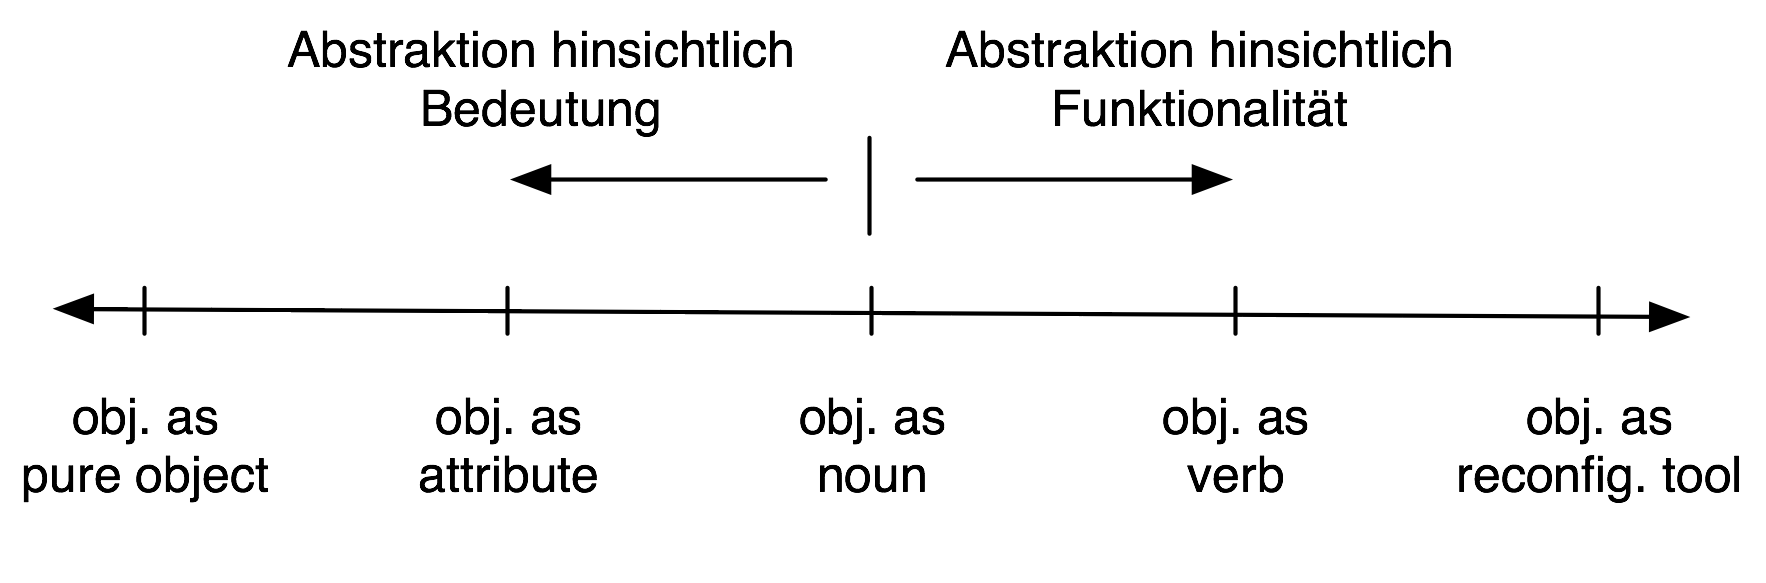
\includegraphics[width=12cm]{img/ImplementierungUeberblick/ObjectMeaning.png}
	\caption[Bedeutung von Objekten in TUIs]{Bedeutung von Objekten in TUIs (adaptiert übernommen aus \citep{Underkoffler99})}
	\label{fig:img_ImplementierungUeberblick_ObjectMeaning}
\end{figure}

\begin{description}
	\item[Object as noun] Derartige Objekte sind Platzhalter für Objekte der realen Welt, denen sie in Form und Verhalten weitgehend entsprechen. Sie stehen für das reale Objekt und werden in dessen Sinne verwendet.
	\item[Object as verb] Die Bedeutung betreffender Objekte reduziert sich auf deren Funktionalität, die Objekte sind nicht mehr Teil der Repräsentation des Systemzustandes sondern werden dazu verwendet, diesen (entsprechend ihrer Funktion) zu verändern.
	\item[Object as reconfigurable tool] Das Objekt wird funktional vollständig von seiner eigentlichen Natur abstrahiert verwendet. Die physischen Eigenschafen stehen nicht mehr in Beziehung zu seiner Verwendung zur Manipulation des Systemzustandes. Die Funktionalität ist dynamisch zuweis- bzw. auswählbar.
	\item[Object as attribute] Objekte werden auf eine ihrer Eigenschaften reduziert. Nur diese wird verwendet, um den Systemzustand abzubilden. Mögliche Eigenschaften sind z.B. Form, Farbe oder Gewicht des Objekts.
	\item[Object as pure Object] Das Objekt wird zum reinen Informationsträger, bei dem die Information nicht in Bezug zur physischen Form oder den Eigenschaften des Objekts steht.
\end{description}

Die Achse beschreibt dabei einen konzeptuelle Ring, der sich an den beiden abstahierten Enden wieder schließt. Einem Objekt, dessen physischen Eigenenschaften keine Rolle im \gls{TUI} mehr spielen, kann beliebig Inhalt oder Funktionalität zugewiesen werden, wodurch die Grenze zwischen linkem und rechtem Ende der Achse verschwimmt.

\begin{tabular}{| p{3cm} | p{10cm} |}
  \hline
  Kategorien & --- \\ \hline
  Konzepte & Object as pure object, Object as attribute, Object as noun, Object as verb, Object as reconfigurable tool  \\ \hline
  Eigenschaften & --- \\ \hline
  PD-Brücke & abhängig von der Art der Tokens  \\ \hline
\end{tabular} 
% subsection tangible_objects_meaning (end)

\subsection{Das MCRpd Interaktions-Modell} % (fold)
\label{sub:mcrpd}

Basierend auf früheren Arbeiten entwickeln \citet{Ullmer00} ein Interaktionsmodell zur Beschreibung von Tangible User Interfaces. Es handelt sich bei dieser Arbeit um den ersten Ansatz, der sich der Domäne aus Sicht der Systemstruktur nähert und nicht ausschließlich eine reine Klassifikation nach bestimmten Merkmalen eines Systems vornimmt.

Die Autoren grenzen \glspl{TUI} von \glspl{GUI} insofern ab, als das \glspl{TUI} über eine nahtlose Integration zwischen Repräsentation des Systemzustandes und dessen Kontrolle aufweisen (im Gegensatz zu \glspl{GUI}, bei denen der Systemzustand über einen graphischen Kanal ausgegeben wird und über andere Kanäle, etwa Tastatur und Maus, kontrolliert wird). Mit der Forderung nach nahtloser Integration von Repräsentation und Kontrolle -- also im Wesentlich einer Einheit von Eingabe- und Ausgabe-Kanälen -- wird ein eher striktes, eingeschränktes Verständnis von \glspl{TUI} propagiert. Als Tangible User Interface kann ein System demnach nur bezeichnet werden, wenn es Ein- und Ausgabe kohärent über einen Kanal führt.


\begin{figure}[htbp]
	\centering
		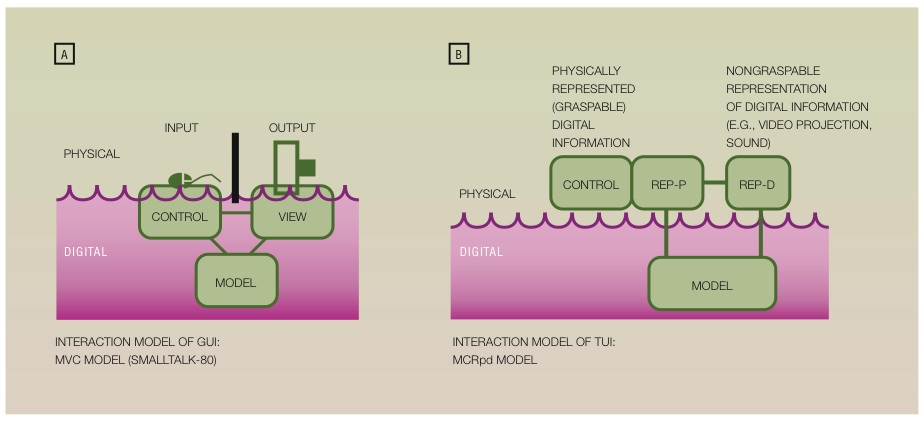
\includegraphics[width=12cm]{img/ImplementierungUeberblick/MCRpd.jpg}
	\caption[Interaktionsmodelle für GUI und TUI]{Interaktionsmodelle für GUI und TUI (übernommen von \citet{Ullmer00})}
	\label{fig:img_ImplementierungUeberblick_MCRpd}
\end{figure}

Diese Sichtweise setzten die Autoren in der Folge in einem Interaktionsmodell für \glspl{TUI} um, dass die Struktur eines Tangible User Interfaces konzeptuell beschreibt. Das Modell wird dabei analog zum \gls{MVC}-Modell konzipiert, das für \glspl{GUI} zum Einsatz kommt und entsprechend der engeren Kopplung zwischen Repräsentation und Kontrolle als \gls{MCRpd}-Modell bezeichnet (siehe Abbildung \ref{fig:img_ImplementierungUeberblick_MCRpd}). An der Gegenüberstellung zwischen \gls{MVC}- und \gls{MCRpd}-Modell wird die Unterscheidung zwischen \gls{GUI} und \gls{TUI} deutlich. Beiden Ansätzen ist gemein, dass der Systemzustand im Rechner durch ein \emph{Model} dargestellt wird. Unterschiede zeigen sich in der Art der Manipulation und Manifestation dieses \emph{Models}. Bei \glspl{GUI} ist Eingabe und Ausgabe strikt getrennt. Die Manipulation des Systemzustandes erfolgt durch die Komponente \emph{Control}, in der physische Kontrollgeräte eine Veränderung des Zustandes erlauben. Die Kontrollgeräte sind dabei im Allgemeinen generisch, d.h. unabhängig vom konkreten Anwendungsfall (also etwa Maus oder Tastatur) und werden durch digitale Kontroll-Elemente an diesen angepasst. Die Ausgabe erfolgt durch die Komponente \emph{View}, wobei auch in diesem Fall ein generisches Ausgabegerät (etwa ein Bildschirm) verwendet wird. Im Falle eines \gls{TUI} existiert keine Trennung zwischen Ein- und Ausgabe. Das \emph{Model} manifestiert sich durch eine \emph{Representation} in der realen Welt. Diese \emph{Representation} hat eine physische Komponente (\emph{REP-P}) und eine digitale Komponente (\emph{REP-D}), die miteinander verknüpft sind. Die digitale Komponente der Repräsentation ist dabei all jene Information, die nicht durch physische, berührbare Elemente dargestellte wird (etwa Projektion, Audio, \ldots). Sie steht dabei jedoch nicht für sich selbst sondern ist immer von eine physischen Repräsentations-Komponente abhängig bzw. dieser zugeordnet. Die physischen Komponenten (\emph{REP-P}) spielen insofern eine zentrale Rolle, als dass ihnen auch die \emph{Control} zugeordnet ist, über sie also der Systemzustand manipuliert werden kann. Die physischen Komponenten des Ausgabe-Kanals fungieren also zugleich als Instanzen des Eingabe-Kanals.

Basierend auf diesem Ansatz identifizieren die Autoren vier Kern-Charakteristika von Tangible User Interfaces:
\begin{itemize}
	\item Physikalische Repräsentationen sind mit digitaler Information gekoppelt
	\item Physikalische Repräsentationen enthalten Mechanismen zur Kontrolle des Systems
	\item Physikalische Repräsentationen sind in der Wahrnehmung der Benutzer mit digitalen Repräsentationen gekoppelt
	\item Der physische Zustand eines Tangible Interfaces stellt die Kernaspekt des Systemzustandes dar
\end{itemize}

Aufbauend auf diesen Eigenschafen entwickeln die Autoren in der Folge ein Schema, das unterschiedliche Ansätze bei der Konzeption eines Tangible Interfaces abdeckt. Als zentrale Ansätze werden „spatial“ (räumliche), „relational“ (relationale) und „constructive“ (konstruierende) Ansätze unterschieden. Räumliche Ansätze nutzen die Anordnung der physischen Elemente in einem Referenzrahmen, um den Systemzustand zu repräsentieren bzw. zu manipulieren. Bei relationalen Ansätzen ist die räumliche Anordnung unwesentlich, lediglich die Beziehungen zwischen den Elementen codieren den Systemzustand. Konstruierende Ansätze sind zwischen den beiden erstgenannten Ansätzen einzuordnen, da sie Beziehungen zwischen Elementen durch eine räumliche Anordnung der Elemente zueinander abbilden. Systeme, in denen Information lediglich in der Zuordnung zu einem physischen Element codiert wird und nicht in der Beziehung zwischen den Elementen, werden in die Kategorie der „associative“ (assoziativen) Ansätze eingeordnet.

Als zusätzliche Gestaltungsdimension führen die Autoren die Konzeption der physischen Repräsentationen an, die bereits in \citep{Ullmer97} eingeführt wurde. Unterschieden wird hier zwischen „iconic“ und „symbolic representations“, wobei ikonische Elemente einen Bezug zu dem jeweils repräsentierten Objekt der realen Welt haben (etwa ein Bild einer Person), während diese Möglichkeit der Zuordnung bei symbolischen Elementen nicht gegeben ist (etwa bei der Repräsentation einer Person durch ein rotes Rechteck). Aus einer umfassenden Betrachtung der zum Zeitpunkt der Erstellung des Artikels verfügbaren Tangible User Interfaces schließen die Autoren, dass ikonische Repräsentationen vorrangig in räumlichen und assoziativen Ansätzen zum Einsatz kommen, während symbolische Repräsentationen eher bei relationen oder konstruierenden Ansätzen anzutreffen sind.

\begin{tabular}{| p{3cm} | p{10cm} |}
  \hline
  Kategorien & spatial, relational, constructive, associative (Einordnung nach Art der Informationsrepräsentation)  \\ \hline
  Konzepte & Model, Rep-P, Rep-D, Control \\ \hline
  Eigenschaften & \emph{Rep-P}: iconic, symbolic \\ \hline
  PD-Brücke & Informationsrepräsentation immer an ein physisches Objekt gebunden. Manipulation der Information erfolgt mittels dem gleichen Objekt \\ \hline
\end{tabular} 

% subsection mcrpd (end)

\subsection{Tokens und Constraints nach Ullmer} % (fold)
\label{sub:tokens_und_constraints_nach_ullmer}

Der Token+Constraint-Ansatz wurde von \citet{Ullmer02} erstmals vorgestellt und \citet{Ullmer05} aktualisiert veröffentlicht. \citeauthor{Ullmer05} gehen dabei erstmals von dem Grundsatz aus, das ein \gls{TUI} zwei grundlegende Arten von physischen Komponenten enthält: Objekte, die digitale Information repräsentieren, und Objekte, die die Interaktion mit Computersystemen bzw. die Manipulation des Systemzustands ermöglichen.

In ihren weiteren Ausführungen identifizieren die Autoren zwei grundlegende Arten von \glspl{TUI}, die sich historisch herausgebildet hätten. Einerseits existieren „interactive surfaces“, bei denen physische Objekte benutzt werden, um Information auf einer aktiven Oberfläche (zumeist projiziert oder durch einen Bildschirm realisiert) zu manipulieren. Andererseits werden „constructive assemblies“ genannt, deren physische Objekte ohne umgebende Infrastruktur ausschließlich durch reale oder logische Verbindungen zwischen ihnen den Systemzustand ausdrücken. Die Autoren definieren nun eine dritte Art von Systemen und platzieren diese konzeptuell zwischen den beiden zuvor genannten Kategorien. Mit „tokens and constraints“ werden Systeme mit zwei unterschiedlichen Arten von physischen Elementen eingeführt. „Tokens“ stehen für Objekte, die digitale Information repräsentieren. „Constraints“ werden verwendet, um (digitale) Funktionalität auf diese Tokens anzuwenden (siehe Abbildung \ref{fig:img_ImplementierungUeberblick_is_tac_ca}).

\begin{figure}[htbp]
	\centering
		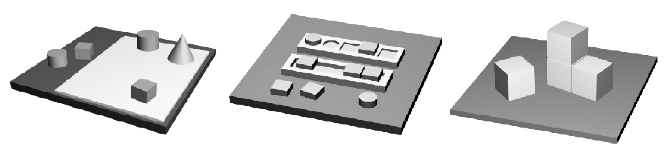
\includegraphics[width=10cm]{img/ImplementierungUeberblick/is_tac_ca.png}
	\caption[Arten von Tangible User Interfaces]{Arten von Tangible User Interfaces -- von links nach rechts: interactive surfaces, tokens+constraints, constructive assemblies (übernommen aus \citet{Ullmer05})}
	\label{fig:img_ImplementierungUeberblick_is_tac_ca}
\end{figure}

In der Folge beschreiben \citeauthor{Ullmer05} die Details des Tokens+Constraints-Ansatzes. Sie gehen dabei zuerst die Benutzer-Interaktion in einem Tokens+Constrains-basieren System. Die ist immer zweigeteilt, wobei in der ersten Phase „associate“ Tokens einem oder mehreren Constraints zugeordnet werden. In der zweiten Phase „manipulate“ werden die Tokens im Kontext der Constraints manipuliert, wodurch die digitalen Daten, die an das Token gebunden sind, geändert werden.

Danach widmen sich die Autoren der Abbildung digitaler Information bzw. deren Manipulation auf physische Elemente und definieren vier grundlegende Arten von Beziehungen, die informationstragend sein können:
\begin{itemize}
	\item die absolute Position eines Tokens in Bezug zu einem Constraint
	\item die relative Position eines Tokens in Bezug zu einem Constraint
	\item die absolute Position eines Tokens in Bezug zu anderen Tokens
	\item die relative Position eines Tokens in Bezug zu anderen Tokens
\end{itemize}
Unter „Position“ sind dabei auch andere spatiale Parameter eines Tokens (wie die Orientierung) zu verstehen.

Nach einer Reihe von Betrachtungen der konzeptuellen Hintergründe und Beispielen kommen die Autoren zu einem weiteren konzeptuell relevanten Punkt, in dem Sie ausführen, wie bzw. warum Tangible Interfaces für Benutzer leichter verständlich sein können als traditionelle \gls{GUI}-basierte Systeme. Bezugnehmend auf \citet{Bellotti02} versuchen Sie Antworten auf fünf von diesen Autoren gestellten Fragen zu finden, die für jede Benutzungsschnittstelle geklärt werden müssen. An dieser Stelle stehen nun nicht die Antworten von \citeauthor{Ullmer05} im Mittelpunkt des Interesses, sondern die Fragen, die einen konzeptuellen Rahmen für das Design einer Benutzungsschnittstelle liefern. Die Fragen stammen aus der Arbeit von \citet{Bellotti02}:
\begin{description}
	\item[Address] Wie weiß das System, dass Benutzer mit ihm und nicht mit anderen (Systemen oder Personen) interagiert?
	\item[Attention] Wie bemerken Benutzer, wenn das System auf eine Interaktionsanforderung reagiert? 
	\item[Action] Wie weiß das System, welchem Objekt der Befehl der Benutzer gilt?
	\item[Alignment] Wie wissen Benutzer, das das System ihren Befehl korrekt verstanden und ausgeführt hat?
	\item[Accident] Wie werden Missverständnisse zwischen den Benutzern und dem System aufgelöst?
\end{description}
\citeauthor{Ullmer05} beantworten diese Fragen für den Tokens+Constraints-Ansatz jeweils aus konzeptueller und technologischer Sicht. 

Am Ende des Artikels geben die Autoren Varianten des Token+Constraints-Ansatzes an. Durch die Festlegung auf die notwendige Physikalität von Tokens und Constraints ist der Design-Raum eingeschränkt, obwohl die konzeptuellen Überlegungen auch breitere Anwendung finden können. Aus diesem Grund variieren die Autoren ihren Ansatz und geben Alternativen an, die den Grundüberlegungen entsprechen aber unter Umständen nicht alle Vorteile des Kernansatzes aufweisen:
\begin{itemize}
	\item Verwendung von visuellen, graphischen Constraints und physischen Tokens
	\item Verwendung von physischen Constraints für graphische Token
	\item Verwendung von physischen Constraints für nicht-massive Tokens (z.B. Flüssigkeiten)
	\item Verwendung von Tokens und Constraints in durch die Benutzer anpassbaren Größen
	\item Alternative Semantik bei der Abbildung zwischen physischer und digitaler Welt
\end{itemize}

Abschließend wird betont, das reife \glspl{TUI} selten in „Reinform“ auftreten, d.h. exakt einer Kategorie wie „interactive surface“ oder „tokens+constraints“ zuzuweisen sind. 

\begin{tabular}{| p{3cm} | p{10cm} |}
  \hline
  Kategorien & interactive surfaces, tokens+constraints, constructive assemblies \\ \hline
  Konzepte & Tokens, Constraints \\ \hline
  Eigenschaften & \emph{Token}: Form, absolute und relative Position in Bezug zu Constraints oder anderen Tokens \\ \hline
  PD-Brücke & Codiert in Tokens und in den Beziehungen zwischen Tokens und Constraints \\ \hline
\end{tabular} 

% subsection tokens_und_constraints_nach_ullmer (end)

\subsection{Degree of Coherence} % (fold)
\label{sub:degree_of_coherence}
\citet{Koleva03} schlagen ein Framework vor, dass die Klassifikation von Tangible Interfaces ermöglichen und so das Verständnis der möglichen Verknüpfungen zwischen physischer und digitaler Welt vertiefen soll. Im Gegensatz zu dem von \citet{Ullmer00} mit dem MCRpd-Modell vorgeschlagenen relative strikten Verständnis eines Tangible Interfaces öffnen \citeauthor{Koleva03} den Begriff und definieren eine kontinuierliche Skala von „Tangibility“, die sich am Grad der „Coherence“ (Kohärenz) zwischen realer und digitaler Welt bemisst. Hohe Kohärenz sagt dabei aus, dass das physische Objekt und sein digitales Gegenstück als ein „Ding“ wahrgenommen werden, also nicht voneinander abgrenzbar sind.

Entlang diesem Kontinuum führen die Autoren Kategorien ein, die die typischen Eigenschaften eines Systems im betreffenden Bereich der Skala beschreiben. Diese Kategorien dienen als Einordnungsschema für Elemente von Tangible Interfaces und können als Grundlage einer Gegenüberstellung unterschiedlicher \glspl{TUI} bzw. deren Komponenten dienen. Entlang der Kohärenz-Skala legen die Autoren folgende Kategorien fest, die sich jeweils auf die Bedeutung des physische Objekt für die Benutzungssschnittstelle beziehen (beginnend mit niedriger Kohärenz): 

\begin{description}
	\item[General-purpose tool] Ein Werkzeug, das zur Manipulation verschiedener digitaler Objekte benutzt werden kann und dabei unterschiedliche Operationen auf diesen Objekten auslösen kann.
	\item[Specialized tool] Ein Werkzeug, das eine bestimmte Operation auslöst, diese aber auf unterschiedliche digitale Objekte anwenden kann.
	\item[Identifier] Objekte, die als Referenz auf ein digitales Objekt agieren. Die Referenz ist nicht zwangsweise permanent sondern kann unter Umständen dynamisch verändert werden.
	\item[Proxy] Objekte, die insofern enger an die digitale Information gekoppelt sind als Identifier, als dass durch sie die digitale Information manipuliert und nicht nur abgerufen werden kann. 
	\item[Projection] Objekte, die so eng an die digitale Repräsentation gebunden sind, dass dessen physische Eigenschaft Information direkt repräsentieren und die Existenz der Information von der Existenz des Objekts abhängig ist.
	\item[Illusion of same objects] Keine Kopplung im engeren Sinne sondern Identität zwischen realem Objekt und digitaler Information. Ist dann gegeben, wenn beide Komponenten ausschließlich gemeinsam auftreten oder für Benutzer nahtlos von der digitalen in die reale Welt und umgekehrt übergehen.
\end{description}

In der Folge detaillieren die Autoren diese Kategorien und identifizieren Eigenschaften, die eine Verknüpfung zwischen realer und digitaler Welt aufweisen kann und an denen sich der Grad an Kohärenz bemisst bzw. an denen er sichtbar wird:

\begin{description}
	\item[Transformation] Beschreibt, wie Manipulationen am realen Objekt in die virtuelle Welt umgesetzt werden. \emph{Literal Mediation} liegt vor, wenn Manipulationen in realer und virtueller Welt analog umgesetzt werden (wenn z.B. eine Bewegung eines Objekts auch in eine Bewegung dessen realer Repräsentation umgesetzt wird). \emph{Transformed Mediation} liegt vor, wenn eine Manipulation eines realen Objekte eine nicht unmittelbar assozierbare Reaktion in der digitalen Welt auslöst (bei der Rotation eines Tokens etwa die Lautstärke eines Audiokanals verändert).
	\item[Sensing of Interaction] Beschreibt auf welche Parameter eines Objektes der realen Welt die digitale Repräsentation reagiert. Die möglichen Ausprägungen reichen von einer binären Reaktion auf die Präsenz eines Objekts bis zur kontinuierlichen Reaktion auf alle sechs Freiheitsgrade des physischen Objekts.
	\item[Configurability of Transformations] Gibt an, ob die Transformation, die zwischen physischem Objekt und digitaler Repräsentation angewandt wird, vorgegeben oder konfigurierbar ist. Mögliche Ausprägungen sind \emph{konfigurierbar} und \emph{fixiert}.
	\item[Lifetime of Link] Gibt an, ob die Assoziation zwischen physischem Objekt und digitaler Repräsentation nach der Kopplung permanent ist oder zur Laufzeit verändert werden kann. Mögliche Ausprägungen sind \emph{temporär} und \emph{permanent}.
	\item[Autonomy] Beschreibt, ob eine Existenzbeziehung zwischen dem realen Objekt und der digitalen Repräsentation besteht, ob also die digitale Ressource unabhängig vom realen Objekt existiert oder bei der Kopplung erzeugt wird. Mögliche Ausprägungen sind \emph{autonom} und \emph{abhängig}.
	\item[Cardinality of Link] Gibt an, ob die Zuordnung zwischen realem Objekt und digitaler Repräsentation eindeutig ist oder ein mehrdeutige Zuordnung von physischer zu digitaler Welt oder umgekehrt möglich ist. Die vorrangig auftretende Ausprägung ist eine eindeutige Abbildung (\emph{1:1}), aber auch \emph{1:n}- oder \emph{n:1}-Abbildungen sind möglich (wobei \emph{n} unbeschränkt oder beschränkt sein kann).
	\item[Link Source] Gibt an, ob der Gegenstand der Manipulation das physische Objekt oder die digitale Repräsentation ist. Die digitale Repräsentation ist dann die Quelle der Kopplung, wenn Änderungen an ihr Auswirkungen auf das physische Objekt haben.
\end{description}

Das hier vorgestellte Framework ist das erste, dass die Art der Verknüpfung zwischen realer und digitaler Welt in das Zentrum der Betrachtung stellt und Tangible User Interfaces entlang dieser Dimension klassifiziert. Die Idee der Berücksichtigung dieses Aspektes bei der Einordnung von \glspl{TUI} wird später von \citet{Fishkin04} (siehe Abschnitt \ref{sub:taxonomie_fishkin}) wieder aufgegriffen und -- vereinfacht -- in seine mehrdimensionale Taxonomie für Tangible User Interfaces integriert.

\begin{tabular}{| p{3cm} | p{10cm} |}
  \hline
  Kategorien & --- \\ \hline
  Konzepte & General-purpose tool, specialized Tool, Identifier, Proxy, Projection, Illusion of same objects \\ \hline
  Eigenschaften & \emph{PD-Brücke}: Transformation, Sensing of Interaction, Configurability of Transformation, Lifetime of Line, Autonomy, Cardinitality of Link \\ \hline
  PD-Brücke & Zentraler Aspekt: Coherence - Maß für die Enge der Bindung zwischen physischem Objekt und digitaler Information (kann für die einzelenen Teile eines Systems unterschiedlich sein) \\ \hline
\end{tabular} 

% subsection degree_of_coherence (end)

\subsection{Tokens und Constraints nach Shaer et al.} % (fold)
\label{sub:tokens_und_constraints_nach_shaer_et_al_}

\citet{Shaer04} stellen in ihrer Arbeit den Anspruch einen Satz von Konstrukten zu identifizieren, der die Struktur und Funktionalität von Tangible User Interfaces zu beschreiben. Letztendliches Ziel ist es, eine konzeptuelle Basis zu schaffen, die die Entwicklung eines Software-Toolkits ermöglicht, das die Spezifikation, Simulation und Implementierung von \glspl{TUI} erlaubt. \citet{Shaer04} bauen dabei auf dem „Token \& Constraints“-Ansatz von \citet{Ullmer02} auf und detaillieren das \emph{Constraint}-Konzept, so dass es die Beschreibung eines \glspl{TUI} vollständiger erlaubt. 

Die grundlegenden Konzepte des Ansatzes orientieren sich an der Annahme, das die Struktur und Funktion eines \gls{TUI} an den Beziehungen zwischen physischen Objekten und digitaler Information festgemacht werden kann. Diese Konzepte sind im Einzelnen:

\begin{description}
 \item[Pyfo] Ein physisches Objekt, das als Teil eines \gls{TUI} eingesetzt wird
 \item[Token] Ein Pyfo, das digitale Information oder eine Funktion zur Veränderung von Information repräsentiert.
 \item[Constraint] Ein Pyfo, das das Verhalten des Tokens, dem es zugeordnet ist, einschränkt. Die physischen Eigenschaften des Constraints weisen auf die Art der Manipulation des Tokens und die Interpretation der Kombination zwischen Token und Constraint hin. Constraints können auf drei Arten einschränkend wirken:
  \begin{itemize}
   \item Die physischen Eigenschaften des Contraints (Form, Material, Orientierung, \ldots) weisen auf die möglichen und nicht erwünschten Manipulationen des zugehörigen Tokens hin
   \item Das Constraint schränkt den physischen Interaktionsraum des Tokens ein
   \item Das Constraint wirkt als Referenzrahmen für das Token und erlaubt dessen Interpretation
  \end{itemize}
 \item[Variable] Digitale Information oder eine Funktion zur Veränderung von Information. Können für sich existieren oder an ein Pyfo gekoppelt sein und dadurch ein Token erzeugen
 \item[TAC] Ein "Token And Constraint" repräsentiert die Beziehung zwischen einem Token, dessen zugeordneter Variable und einem oder mehreren Constraints. \glspl{TAC} legen fest, wie Benutzer mit dem System interagieren können
\end{description}

Basierend auf diesen Konzepten werden fünf Kerneigenschaften, die ein Tangible User Interface bzw. dessen Elemente aufweisen können. Diese Kerneigenschaften sind:

\begin{description}
	\item[Couple] Ein Pyfo muss an eine Variable gekoppelt sein, um als Token zu gelten
	\item[Relative Definition] Jedes Pyfo muss ein Token, ein Constraint oder beides sein
	\item[Association] Ein \gls{TAC} bildet sich aus der physischen Zuordnung eines Tokens zu einem Constraint. Dem \gls{TAC} können weitere Constraints zugeordnet werden
	\item[Computational Interpretation] Physische Manipulation eines Tokens hat eine eindeutig interpretierbare Auswirkung auf die digitale Welt
	\item[Manipulation] Jedes \gls{TAC} kann in der physischen Welt diskret, kontinuierlich oder auf beide Arten manipuliert werden. Das Constraint legt die möglichen Arten der Manipulation fest.  
\end{description}

Zur Spezifikation eines Tangible User Interfaces werden nun diese Konzepte zur Anwendung gebracht um sowohl Struktur als auch Verhalten des \gls{TUI} festzulegen. Bei der Spezifikation werden die \glspl{TAC} definiert, indem auf Seiten der Struktur das betroffene Token und die zugehörigen Constraints angeführt werden. Zur Spezifikation des Verhaltens wird die betroffene Variable, die Aktion, die in der physischen Welt ausgeführt wird und die zu erwartende Reaktion des Systems angeführt.

\begin{tabular}{| p{3cm} | p{10cm} |}
  \hline
  Kategorien & --- \\ \hline
  Konzepte & Pyfo, Token, Constraint, Variable, \gls{TAC} \\ \hline
  Eigenschaften & Couple, Relative Definition, Association, Computational Interpretation, Manipulation \\ \hline
  PD-Brücke & Variables (Elemente der digitalen Welt) machen ein Pyfo (Objekt der realen Welt) zu einem Token \\ \hline
\end{tabular} 

% subsection tokens_und_constraints_nach_shaer_et_al_ (end)

\subsection{Kategorien von TUI-Anwendungen} % (fold)
\label{sub:kategorien_von_tui_anwendungen}

Auf Basis einer umfassenden Literaturrecherche im Bereich von interaktiven Systemen, bei denen physische Objekte zur Interaktion und Informationseingabe benutzt werden, identifizieren \citet{Klemmer04} vier Kategorien von Ansätzen, die bei der Umsetzung eines \gls{TUI} verfolgt werden können. 

\begin{description}
	\item[Spatial Applications] Applikationen, bei denen die Interaktion auf einer beliebigen Oberfläche (Wände, Tische, Whiteboard, \ldots) abgewickelt wird und Information über diese Oberfläche dargestellt und manipuliert werden kann. Dazu gehören auch Systeme, die ohne physische Elemente (neben der Oberfläche) arbeiten.
	\item[Topological Applications] Applikationen, bei denen die Kontrolle des Systems über die Herstellung von Beziehungen zwischen physischen Objekten durchgeführt wird.
	\item[Associative Applications] Applikationen, bei denen physische Objekte als Referenz auf digitale Information fungieren und diese durch Interaktion mit einer Hintergrund-Infrastruktur abgerufen werden kann.
	\item[Forms] Applikationen, bei denen papierbasierte Interaktionen zu einem bestimmten Zeitpunkt (nicht kontinuierlich) in die digitale Welt übernommen werden (z.B. durch Scannen und \gls{OCR}-Verarbeitung).
\end{description}

Die Autoren gehen nicht weiter ins Detail und verzichten auf eine Betrachtung der unterschiedlichen Eigenschaften des Systems. Sie geben lediglich an, dass die meisten der betrachteten Applikationen Gemeinsamkeiten über die Grenzen der Applikationskategorien hinweg. Dies umfasst die Tatsache, dass das vorherrschende Systemdesign die Verbindung zwischen physikalischer (tangibler) Eingabe und graphischer Ausgabe ist. Die graphische Ausgabe erfolgt dabei entweder kohärent mit der Eingabe (auf der gleichen Oberfläche), auf einem separaten Bildschirm, der sich aber nahe dem Eingabemedium befindet oder entfernt auf von den eingebenden Benutzern nicht unmittelbar zugreifbaren Ausgabemedien. Interfaces, die die Ausgabe auf andere Arten (z.B. haptisch) gestalten, werden von den Autoren explizit vernachlässigt, da sie für die eigene Forschung keine Relevanz haben.

\begin{tabular}{| p{3cm} | p{10cm} |}
  \hline
  Kategorien & Spatial, Topological, Associative, Forms \\ \hline
  Konzepte & --- \\ \hline
  Eigenschaften & --- \\ \hline
  PD-Brücke & --- \\ \hline
\end{tabular} 

% subsection kategorien_von_tui_anwendungen (end)

\subsection{Taxonomie nach Fishkin} %(fold)
\label{sub:taxonomie_fishkin}

\citet{Fishkin04} versucht in seiner Arbeit, den Begriff des Tangible User Interfaces zu definieren und ein Kategorienschema zu schaffen, in das sich auf tangibler Interaktion beruhende Systeme einordnen lassen. Sein Ziel ist es, ein Framework zur Verfügung zu stellen, auf Basis dessen sich Systeme vergleichen lassen und das das Design von Tangible Interfaces unterstützen kann.

\citeauthor{Fishkin04} fasst den Begriff des Tangible Interfaces sehr breit und definiert ein Interaktives System mit tangiblem Interface als eines, in dem die Eingabe über die Manipulation (im wörtlichen Sinn, also mit den Händen) von phyischen Objekten vorgenommen wird und die Ausgabe die physische Natur eines Objektes verändert. Diese Definition umfasst auch Systeme mit "herkömmlichen" Interfaces.

Nach dieser umfassenden Definition strukturiert \citeauthor{Fishkin04} den Raum möglicher Tangible Interfaces durch die Einführung zweier Analysedimensionen, anhand derer er seine  Taxonomie aufspannt. Diese beiden Dimensionen sind "Embodiment" und "Metaphor". Sie sind orthogonal zueinander und hohe Wert dieser beiden Dimensionen bezeichnen "tangiblere" Systeme. "Hohe Tangibilität" ist jedoch kein Qualitätskriterium sondern lediglich eine Eigenschaft, die ein System für einen bestimmten Anwendungsfall besser oder schlechter geeignet machen kann.

\subsubsection{Embodiment}
Die Dimension "Embodiment" beschreibt, wie eng die Eingabe am Interface mit der Ausgabe gekoppelt ist. Das Kriterium zu Einordnung ist hier der Ort der Wahrnehmbarkeit des Systemzustandes und der Systemaktivität. Je kohärenter die Ausgabe- und Eingabe-Kanäle sind, je näher sich die Informationsausgabe also bei der Eingabe befindet, desto höher ist die Ausprägung dieser Dimension. \citeauthor{Fishkin04} unterscheidet hier vier Ausprägungen:
\begin{description}
 \item[Full] Bei "full Embodiment" ist das Ausgabegerät gleichzeitig das Eingabegerät. Der Zustand des Geräts ist direkt in seinen physischen Eigenschaften abgebildet.
 \item[Nearby] "Nearby Embodiment" tritt auf, wenn die Ausgabe nahe dem Eingabeobjekt auftritt und eng an dieses gebunden ist, also in direktem, unmittelbaren Zusammenhang steht. 
 \item[Environmental] "Environmental Embodiment" ist gegeben, wenn die Ausgabe im unmittelbaren Umfeld des auftritt aber sich nicht unmittelbar am tangiblen Eingabeobjekt manifestiert. Typische Vertreter dieser Ausprägung sind akustische Ausgabekanäle.
 \item[Distant] Von "distant Embodiment" spricht man, wenn sich Ein- und Ausgabekanäle vollständig räumlich entkoppelt sind, der Fokus der Aufmerksamkeit der Benutzer also nicht gleichzeitig auf Ein- und Ausgabekanal liegen kann. 
\end{description}

\subsubsection{Metaphor}

Die Dimension "Metaphor" bildet die Eigenschaft von Tangible Interfaces ab, auf eine Benutzerinteraktion so zu reagieren, wie die reale Welt auf eine entsprechende Aktion reagieren würde. Die Ausprägung in "Metaphor" ist also dann hoch, wenn das System analog zu realem, physikalisch begründbarem Verhalten reagiert. Hier sind grundsätzlich zwei Kategorien zu unterscheiden, in denen der Bezugspunkt der "Methaphor" verschieden ist. "Metaphor" kann sich entweder auf das Aussehen des jeweiligen Objektes beziehen oder auf die Bewegung des Objektes Bezug nehmen. Im ersten Fall spricht \citeauthor{Fishkin04} von "Metaphor of Noun", im zweiten Fall von "Metaphor of Verb". Die Ausprägungen auf der "Metaphor"-Dimension gruppieren sich dann wie Folgt:
\begin{description}
 \item[None] Die Interface-Objekte zeigen weder in Form noch Funktion eine Analogie zur Realität
 \item[Noun] Diese Analogie ist gegeben, wenn am Interface Objekte existieren, die eine reale Entsprechung haben, aber nicht wie diese manipuliert werden können. Ein klassisches Beispiel aus traditionellen interaktiven Systemen ist die "Fenster"- oder "Schreibtisch"-Metapher (sind analog zu realen Fenstern bzw. Schreibtischen ausgelegt, bieten aber andere Interaktionsmöglichkeiten). Bei Tangible User Interfaces ist diese Zuordnung dann gegeben, wenn ein Eingabeobjekt so aussieht wie ein Objekt der realen Welt, aber keine weiteren Eigenschaften mit diesem teilt.
 \item[Verb] Eine Zuordung zu dieser Kategorie erfolgt, wenn die Interaktion mit einem Objekt eine reale Entsprechung hat, dieses jedoch selbst keine Analogie zur realen Welt bildet. Diese Ausprägung tritt bei \glspl{TUI} unter anderem bei Gestensteuerung von Systemen auf.
 \item[Noun and Verb] Hier hat das betreffende Objekt selbst eine Entsprechung in der realen Welt und auch dessen Verwendung ist analog zu jener der realen Entsprechung. Die Objekte sind dennoch nach wie vor unterschiedlich, das reale Objekt kann nicht im Tangible Interface eingesetzt werden, umgekehrt bietet das \gls{TUI}-Objekt nicht die reale Funktionalität des realen Objektes. 
 \item[Full] In der höchsten Ausprägung existiert kein Unterschied zwischen \gls{TUI}-Objekt und realem Objekt - es gibt keine Analogie mehr, weil die Objekte identisch sind. Dieser Zustand ist erreicht, wenn Benutzer das TUI-Objekt manipulieren und sich die reale Welt entsprechend verändert. Beispiele für Systeme auf dieser Stufe sind zum Beispiel digital augmentierte Whiteboards, wo mit elektronischen Markern auf eine Oberfläche "geschrieben" wird, wobei die hinterlassene "Tinte" simultan projiziert wird.
\end{description}

\subsubsection{Anwendung der Taxonomie}
\citeauthor{Fishkin04} wendet seine Taxonomie auf die oben bereits beschriebenen Ansätze von \citep{Holmquist99} und \citep{Underkoffler99} an und zeigt, dass sich diese einordnen lassen. Er ordnet nach einer umfassenden Literaturstudie außerdem über 60 konkrete Tangible Interfaces in seine Taxonomie ein und stellt diese anhand deren Ausprägungen gegenüber. Ein offener Punkt ist die Verbindung zum \gls{MCRpd}-Framework \citep{Ullmer00}, dass \citeauthor{Fishkin04} als komplementär bezeichnet und das auf einer anderen Abstraktionsstufe operiere. 

\begin{tabular}{| p{3cm} | p{10cm} |}
  \hline
  Kategorien & --- \\ \hline
  Konzepte & --- \\ \hline
  Eigenschaften & \emph{Embodiment}: full, nearby, environmental, distant, \emph{Metaphor}: none, noun, verb, noun and verb, full\\ \hline
  PD-Brücke & wird in Struktur und Verhalten durch die Ausprägungen auf den beiden Dimensionen der Taxonomie charakterisiert (kann für die einzelnen Teile eines Systems unterschiedlich sein)  \\ \hline
\end{tabular} 

% subsection taxonomie_fishkin (end)

\subsection{Mixed Reality} % (fold)
\label{sub:mixed_reality}

% subsection mixed_reality (end)

\subsection{Tangible Bits: Beyond Pixels} % (fold)
\label{sub:tangible_bits_beyond_pixels}

\citeauthor{Ishii08} fasst in \citep{Ishii08} die bisherige Entwicklung des Forschungsgebiets der Tangible User Interfaces zusammen und schlägt konzeptuell die Brücke von den wegweisenden \emph{Tangible Bits}-Arbeiten über das MCRpd-Interaktions-Modell bis hin zu heute aktuellen Kategorien von Tangible User Interfaces.

Die Grundlage der Betrachtungen ist das in \citep{Ullmer00} MCRpd-Interaktions-Modell, das hier (und bereits in \citep{Ullmer05}) als \gls{MCRit}-Modell bezeichnet wird. („it“ für „intangible“ und „tangible“ anstatt „physical“ und „digital“). Basierend auf der Trennung zwischen Input und Output eines interaktiven Systems (oder \emph{Control} und \emph{Representation}) und der auf dieser Trennung aufbauenden Abgrenzung zur \glspl{GUI}, wird die Struktur eine \gls{TUI} so konzeptualisiert, das eben diese Trennung nicht mehr vorhanden ist. Die grundlegenden Komponenten des \gls{MCRit}-Modells sind (angelehnt an das \gls{MCRpd}-Modell) die \emph{digitale Information}, die repräsentiert und manipuliert werden muss, sowie die \emph{tangible Repräsentation} des Systemzustandes (siehe Abbildung \ref{fig:img_ImplementierungUeberblick_MCRit}). An die tangible Repräsentation sind die Eingabekanäle des Systems -- die \emph{Control} -- gekoppelt. Die tangible Repräsentation wird durch die intangible Repräsentation ergänzt, mittels der zusätzliche, dynamisch veränderliche Information abhängig vom Systemzustand ausgegeben werden kann.

\begin{figure}[htbp]
	\centering
		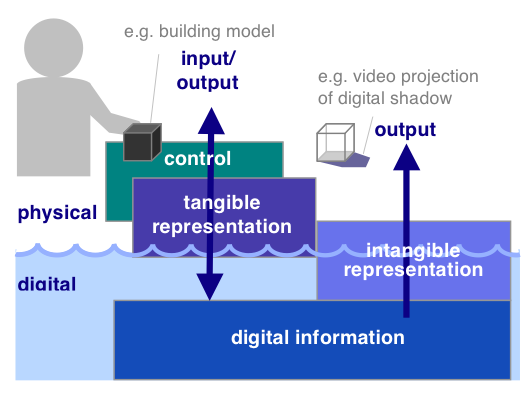
\includegraphics[height=3in]{img/ImplementierungUeberblick/MCRit.png}
	\caption{caption}
	\label{fig:img_ImplementierungUeberblick_MCRit}
\end{figure}

Basierend auf der konzeptuellen Grundlage gibt \citeauthor{Ishii08} die grundlegenden Eigenschaften von \glspl{TUI} an:
\begin{description}
	\item[Computational Coupling] \emph{of tangible representations to underlying digital information and computation}. Der zentrale Aspekt jedes \gls{TUI} ist die Kopplung von realen Artefakten mit digitaler Information und diese Information manipulierende Funktionen. Zu berücksichtigen ist dabei die Art der Abbildung, also welche Prinzipien der Übersetzung und welche Metaphern (bei \citeauthor{Ishii08}: "Embodiment") verwendet werden.
	\item[Embodiment of mechanisms for interactive control] \emph{with tangible representations}. In \glspl{TUI} werden die physischen Repräsentationen des Systemzustandes gleichzeitig auch zur Steuerung des Systems verwendet. Von Interesse sind hier die Fähigkeiten des Tangibles selbst ("inert", also passive Objekt, die durch Benutzer manipuliert werden müssen oder "actuated", also aktive Elemente, die selbständig Änderungen des Systemzustandes ausgeben können), die Beschränkung des Interaktionsraums ("unconstrainted" -- unbeschränkt, "weakly constrainted" -- nur schwach eingeschränkt, wie bei der Interaktion auf Oberflächen, oder "tightly constrainted" -- stark eingeschränkt, z.B. bei Tokens die nur entlang einer Achse bewegt werden können) sowie die durch die physische Form der Tokens und die Constraints vorgegebenen bzw. angedeuteten Interaktionen und deren Kohärenz mit der dadurch manipulierten digitalen Information.
	\item[Perceptual Coupling] \emph{of tangible representations to dynamic intangible representations}. Die wahrgenommene Kopplung zwischen dem physischen Anteil des Systemzustandes und dem intangiblen (z.B. projizierten oder akustischen) Anteil ist der dritte wichtige Aspekt, der beim Design von Tangible Interfaces zu berücksichtigen ist. Der kritische Faktor ist dabei nach \citeauthor{Ishii08} die Reaktion des intangiblen Anteil auf Änderung des tangiblen Anteils in Echtzeit. Zwischen der Manipulation von physischen Elementen und eine adäquaten Reaktion des Systems, die sich auch auf die intangible Repräsentation auswirkt, darf nur minimale, idealerweise nicht als solche wahrgenommene Verzögerung liegen. 
\end{description}

Je nach Ausprägung dieser Eigenschaften können sich \glspl{TUI} in unterschiedliche Kategorien von Systemen manifestieren. Basierend auf den bereits in \citep{Ullmer05} angegebenen Kategorien erweitert \citeauthor{Ishii08} das Schema und identifiziert acht Kategorien von \glspl{TUI}:
\begin{description}
	\item[Tangible Telepresence] Systeme, bei denen entfernte physische Objekte digital miteinander gekoppelt werden, so dass Manipulationen eines Objekts an den gekoppelten Objekten physisches Feedback auslösen können. Durch die Kopplung zwischen entfernter Ein- und Ausgabe können Präsenz-Aspekte auch in dissoziierten Anwendungsfällen übermittelt werden.
	\item[Tangibles with kinetic Memory] Systeme, die Manipulation physischer Objekte aufnehmen und diese Manipulationen auch wieder physisch wiedergeben können.
	\item[Constructive Assembly] Entspricht der in \citep{Ullmer05} angegebenen Kategorie und umfasst Systeme, bei denen der Systemzustand durch die (physische) Verknüpfung von physischen Elementen repräsentiert und manipuliert wird.
	\item[Tokens and Constraints] Entspricht der in \citep{Ullmer05} angegebenen Kategorie und umfasst Systeme, die informationstragende physische Elemente zur Repräsentation des Systemzustandes benutzen und die möglichen Interaktionen mittels ebenfalls physischer Constraints beschränken bzw. vorgeben.
	\item[Interactive Surfaces -- Tabletop UI] Entspricht der in \citep{Ullmer05} angegebenen Kategorie und umfasst Systeme, bei denen physische Objekte auf einer Oberfläche manipuliert werden, um den Systemzustand zu verändern. Dabei wird meist zusätzlich visuelles Feedback auf der Oberfläche ausgegeben, wodurch Eingabe- und Ausgabemedium kohärent sind.
	\item[Continuous Plastic TUI] Umfasst Systeme, die in der Lage sind, die äußere Form ihrer physischen Repräsentationen zu verändern bzw. auf derartige Formänderungen mit Änderungen des Systemzustandes reagieren.
	\item[Augmented Everyday Objects] Systeme, bei denen physische Objekte des Alltagslebens mit Technologie ausgestattet wird, die einen wie auch immer gearteten Mehrwert bei der Benutzung bieten kann.
	\item[Ambient Media] Systeme, bei denen interaktive Systeme durch Zusatzinformation ergänzt werden, die nicht von der eigentlichen Arbeitsaufgabe ablenken. Im engeren Sinne handelt es sich dabei nach \citeauthor{Ishii08} nicht um ein \gls{TUI}, die Kategorie hat aber insofern Relevanz, als dass nicht die herkömmlichen Ausgabekanäle (wie Bildschirme) benutzt werden, um digitale Information zu repräsentieren.
\end{description}

Grundlegend gemein sind jedoch allen Arten von Systemen ein Satz von Merkmalen, die sie in ihrer Eigenschaft als \glspl{TUI} mitbringen und die sich dem Autor zufolge durchwegs vorteilhaft auf die Interaktion mit den Benutzern auswirken können:
\begin{description}
	\item[Double Interaction Loop -- Immediate Tactile Feedback] Tangible User Interfaces verfügen inhärent über zwei Feedbackschleifen über die den Benutzern Reaktionen auf deren Eingaben rückgespiegelt werden. Die erste, unmittelbar, Feedback-Schleife ist die haptische Erfahrung bei der Manipulation der physischen Element. Die Reaktion ist sofort sichtbar und muss nicht durch das System erfasst, interpretiert und ausgegeben werden. Die zweite Schleife wird über die intangible Repräsentation des Systemzustands realisiert, auf der sich ebenfalls Reaktionen auf Benutzereingaben manifestieren. Dabei muss die Benutzerinteraktion jedoch erfasst und interpretiert werden, bevor eine adäquate Reaktion erstellt und ausgegeben werden kann. Diese Reaktion kann umfassender als in der ersten Schleife ausfallen, benötigt jedoch mehr Zeit.
	\item[Persistency of Tangibles] Bei \glspl{TUI} wird ein wesentlicher Anteil des Systemzustandes durch die Konfiguration des physischen Elemente dargestellt. Diese sind ihrer Natur nach persistent, repräsentieren diesen Anteil des Systemzustandes also unabhängig von etwaiger Infrastruktur und sind auch verfügbar, wenn diese abgeschaltet ist.
	\item[Coincidence of Input and Output Spaces] Ein grundlegendes Designkriterium von \glspl{TUI} ist die Kohärenz (bei \citeauthor{Ishii08}: Koinzidenz) von Eingabe- und Ausgabekanälen. Dies ermöglicht eine nahtlose Interaktion und Informationsrepräsentation im physischen und digitalen Raum. 
	\item[Special Purpose vs. General Purpose] In Abgrenzung zu \glspl{GUI}, die im Normalfall zur Interaktion mit beliebigen Applikationen verwendet werden können, sind \glspl{TUI} eher spezifisch auf einen bestimmten Anwendungsfall hin ausgerichtet und und werden dementsprechend konzipiert. Wichtig ist hier vor allem die Berücksichtigung den Benutzern vertrauter Metaphern bei der Konzeption der Informationsrepräsentation und der Manipulations-Werkzeuge.
	\item[Space-Multiplexed Input] Generell ermöglichen \glspl{TUI} eine parallele Manipulation mehrerer räumlich verteilter physischer Objekte zur gleichen Zeit. Es ist damit möglich, kollaborative Interaktion zu unterstützen, bei der mehrere Benutzer den Systemzustand simultan beeinflussen. Die Kollaboration kann dabei auch räumlich verteilt stattfinden, wenn Mechanismen existieren, die den Systemzustand der einzelnen \gls{TUI}-Instanzen synchron hält (z.B. durch Aktuatoren). 
\end{description}

Im seinen Schlussbetrachtungen führt \citeauthor{Ishii08} die größten Mängel des noch jungen Forschungsgebiets der Tangible User Interfaces aus: es fehle an „Killer Applications“, an skalierbaren Toolkits und an verlässlichen und validierten Design Prinzipien.

\begin{tabular}{| p{3cm} | p{10cm} |}
  \hline
  Kategorien & Tangible Telepresence, Tangibles with kinetic Memory, Constructive Assembly, Tokens and Constraints, Interactive Surfaces -- Tabletop UI, Continuous Plastic TUI, Augmented Everyday Objects, Ambient Media \\ \hline
  Konzepte & Digital Information, Tangible Representation, Control, Intangible Representation \\ \hline
  Eigenschaften & \emph{Gesamtsystem}: Computational Coupling, Embodiment of Control Mechanisms, Perceptual Coupling \\ \hline
  PD-Brücke & Abhängig von der Art des Systems, grundsätzlich aber immer Kopplung zwischen tangibler Repräsentation und Control \\ \hline
\end{tabular} 

% subsection tangible_bits_beyond_pixels (end)

\subsection{Zusammenfassung} % (fold)
\label{sub:tui_konzepte_zusammenfassung}

Die in den vorhergehenden Abschnitten betrachteten Arbeiten sind in Ansatz, Ausgangspunkt und Vorgehensweise höchst unterschiedlich, ihnen ist jedoch gemein, dass sie sich mit der Konzeptualisierung von Tangible User Interfaces beschäftigen. Die Arbeit können dabei entlang zweier Dimensionen nach Ziel und Betrachtungsgegenstand klassifiziert werden. Hinsichtlich der Zielsetzung sind Arbeiten, die auf die Spezifikation eines \gls{TUI} ausgerichtet sind von solchen zu unterscheiden, die auf die Evaluation existierender Systeme ausgelegt wurden (im Sinne von detailliert angegebenen Merkmalen, die ein System aufweisen muss, um eine bestimmte Eigenschaft zu haben). Als dritte Ausprägung sind noch Ansätze zu identifzieren, die eine Einordnung in einen Referenzrahmen ermöglich sollen ohne die Eigenschaften des Hinsichtlich des \gls{TUI} im Detail zu betrachten. Betrachtungsgegenstandes sind unterschiedliche Detaillierungsgrade zu erkennen, wobei hier die beiden Ausprägungen "Gesamtsystem" und "einzelne physische Elemente" als Extremwerte zur Klassifikation herangezogen werden. Hinsichtlich des Betrachtungsgegenstandes ist noch zu unterscheiden, ob sich die Arbeit auf die Struktur des \gls{TUI} konzentriert oder sich darüber hinaus auch explizit mit dessen Verwendung beschäftigt. Ansätze der zweiten Art werden in der Tabelle kursiv gesetzt. Jeder Ansatz verfolgt über diese Einordnung hinaus noch spezifische Zielsetzungen, die der Übersicht wegen in dieser ersten Einordnung nicht angegeben werden. 

Die Einordnung in die Kategorien (siehe Tabelle \ref{tab:tui_konzeptkategorien}) erfolgt aufgrund der von den jeweiligen Autoren in den Artikeln explizit genannten Zielsetzungen oder -- wenn diese nicht vorhanden oder aussagekräftig sind -- aufgrund der von Autoren gewählten Schwerpunktsetzungen und unter Berücksichtigung des jeweiligen Gesamtzusammenhangs (übergeordnetes Forschungsvorhaben). Ansätze, die zu mehreren Kategorien Beiträge liefern, werden in allen betreffenden Feldern angeführt.

\begin{table}[htbp]
	\centering
	\caption{Kategorien von konzeptuellen Arbeiten im Gebiet Tangible User Interfaces}
	\begin{tabular}{| p{2,5cm} || p{5,5cm} | p{5,5cm} |} \hline
		 & Gesamtsystem & einzelne physische Elemente \\ \hline \hline
		Spezifikation & Bricks\linebreak MCRpd-Interaktions-Modell\linebreak Tangible Bits: Beyond Pixels & Containers, Tokens und Tools\linebreak Tokens+\-Constraints\linebreak \emph{Tokens and Constraints nach Shaer et al.}\\ \hline
		Evaluation & Graspable User Interfaces & \emph{Taxonomie nach Fishkin} \\ \hline
		Einordnung & Tangible Bits\linebreak Tokens+\-Constraints\linebreak Kategorien von TUI Anwendungen\linebreak Tangible Bits: Beyond Pixels & Tangible Objects Meaning\linebreak Degree of Coherence \\ \hline
	\end{tabular}
	\label{tab:tui_konzeptkategorien}
\end{table}

In dieser Aufstellung ist zu erkennen, dass eine Großteil der Ansätze nicht auf den  Interaktionsaspekt des Anwendungsfalls eingeht, für den das betrachtete \gls{TUI} konzipiert ist, sondern sich auf die sturkturellen Aspekte des Systems beschränkt.  

Den umfassendsten Ansatz zur Spezifikation bietet die Arbeit "Tokens and Constraints" von \citep{Shaer04}, der aufbauend auf der Arbeit von \citet{Ullmer02} einen modifizierten Token+Constraints-Ansatz vorstellt, der sich durch ein breiteres Verständnis des Constraint-Begriffs für die allgemeine Spezifikation der Struktur eines TUI eignet und zusätzlich ein Schema zur Verfügung stellt, in dem basierend auf der Struktur das Verhalten des Systems spezifiziert werden kann.

Zur detaillierten Evaluation eines \gls{TUI} bietet sich die Taxonomie von \citet{Fishkin04} an, der in seiner Arbeit in zwei Dimensionen sowohl die Betrachtung der Struktur als auch der Verwendung der Objekte eines \gls{TUI} in den spezifizierten Interaktionsabläufen erlaubt.

\subsubsection{Ausdrucksstärke der konzeptuellen Ansätze} % (fold)
\label{ssub:ausdrucksstärke_der_konzeptuellen_ansätze}

Grundsätzlich sind jene Ansätze, die sich mit der detaillierten Beschreibung eine \gls{TUI} befassen, ausdrucksstärker als jene Ansätze, die ein System lediglich global betrachten. Dies bezieht sich jedoch in erster Linie auf die Quantität der generierten Daten, qualitativ gesehen ergänzen beide Sichtweisen einander und sind sowohl bei Spezifikation als auch Evaluation komplementär anzuwenden. Der Fokus der Betrachtung der jeweiligen Ansätze ist in Tabelle \ref{tab:tui_konzeptkategorien} angeführt und wird hier nicht separat unterschieden.

Einige der vorgestellten Ansätze sind inhaltich insofern als überholt anzusehen, als dass sie heute gängige Techniken und Interaktionsparadimen nicht adäquat abbilden können. Dies gilt sowohl in struktureller Hinsicht als auch in Bezug auf das Verhalten eines Systems. Die strukturellen Konzepte haben sich konzeptuell von "werkzeug-zentrierten" auf "informations-zentrierte" Sichtweise weiter entwickelt. Ältere, "werkzeug-zentrierte" Ansätze betrachten die physischen Elemente ausschließlich als Werkezeuge zur Manipulation digitaler Information, die nach wie vor herkömmlich visuell ausgegeben wird und keine physische Manifestation besitzt. Typische Vertreter dieser Sichtweise sind \citep{Fitzmaurice95} und \citep{Fitzmaurice96}. Ab der Arbeit von \citet{Ishii97} wird der Aspekt der physischen Repräsentation von Information berücksichtigt, womit erstmals eine umfassende Beschreibung von Systemen ermöglicht wird, die heute als \gls{TUI} bezeichnet werden.

In der Folge wurden unterschiedliche Ansätze vorgestellt, die auf unterschiedliche Aspekte in der Beschreibung der Struktur eingehen. Ein grundlegendes Unterscheidungsmerkmal der Ansätze ist ihre Herangehensweise an die Unterscheidung zwischen physischen Objekten, die Information repräsentieren und solchen, die Information manipulieren (in wenigen Fällen werden auch Werkzeuge zur Systemsteuerung separat betrachtet). Eine Herangehensweise ist die strikte konzeptuelle Trennung zwischen physischen Objekten, die zur Informationsrepräsentation verwendet werden und sochen, die als Werkzeug zur Manipulation eingesetzt werden. Typische Verterter sind hier \citep{Ishii97} und \citep{Holmquist99}. Dem hingegen steht die Herangehensweise, die Bedeutung eines physischen Objekts für eine bestimmte Anwendung auf einem Kontinuum einzuordnen und Objekte damit als eher "werkzeug-artig" oder eher "repräsentations-artig" (oder beides integrierend) einzuordnen. Typische Vertreter für diese Herangehensweise sind \citep{Underkoffler99}, \citep{Koleva03} und \citep{Fishkin04}. Einen dritten Weg gehen die Ansätze von \citep{Ullmer00} und darauf aufbauend \citep{Ishii08}, die physische Elemente immer als Kombination eines Repräsentations- und Kontroll-Anteils sehen und diese konzeptuell separat behanden. Implzit in dieser Tradition stehen auch die Ansätze von \citep{Ullmer02} und \citep{Shaer04}, die mit dem "Tokens und Constraints"-Konzept einerseits eine dritte Art von physischen Objekten -- die Constraints, die den Interaktionsraum beschränken -- einführen, andererseits aber bei den eigentlich zur Interaktion verwendeten physischen Elementen nicht zwischen Repräsentationen und Werkzeugen unterscheiden. Funktionalität wird vielmehr durch die Manipulation eines (informationstragenden) Tokens im Kontext von Constraints ausgelöst -- Tokens haben somit einen Kontroll-Aspekt im Sinne von \citep{Ullmer00}.

Weniger häufig anzutreffen sind Arbeiten, die explizit auf die Beschreibung oder Evaluation der Interaktionsabläufe eines \gls{TUI} eingehen. TODO

% subsubsection ausdrucksstärke_der_konzeptuellen_ansätze (end)

\subsubsection{Nomenklatur}

Hinsichtlich der Bezeichnung der Elemente eines \gls{TUI} existiert keine einheitliche Nomenklatur, die konsistent über mehrere Arbeiten hinweg verwendet werden würde. Tabelle \ref{tab:tui_nomenklatur} gibt eine Übersicht über die für die einzelnen konzeptuellen Elemente verwendeten Begriffe.

\begin{longtable}{| p{1,9cm} || p{1,8cm} | p{2,4cm} | p{2,4cm} | p{1,8cm} | p{1,8cm} |} 
	\caption{Gegenüberstellung der Nomenklatur zur Beschreibung der Elemente eines TUI} \label{tab:tui_nomenklatur} \\
	\hline
	Ansatz & physisches Objekt & physisches Objekt zur Informations\-repräsentation & physisches Werkzeug zur Informations\-manipulation & physische Beschränkung des Interaktionsraums & digitale Objekte \\ \hline \hline
	Bricks & --- & --- & Brick & --- & --- \\ \hline
	Graspable User Interfaces & --- & --- & --- & --- & --- \\ \hline
	Tangible Bits & --- & Phicon & Phandle (Informationsmanipulation), Instrument (Systemsteuerung) & Tray & --- \\ \hline
	Containers, Tokens und Tools & --- & Container (unspezifische Form), Token (spezifische Form) & Tool & --- & --- \\ \hline
	Tangible Objects Meaning & Object & Object as pure object (unspezifische Form), Object as attribute (teilspezifisch), Object as noun (spezifische Form) & Object as verb (fix gebundene Funktionalität), Object as reconfigurable tool (konfigurierbare Funktionalität) & --- & --- \\ \hline
	MCRpd Inter\-aktions-Modell & Represen\-tation & Rep-P & Control & --- & Model, Rep-D (Manifestation)\\ \hline
	Tokens+\-Constraints & --- & Tokens & Tokens+\-Constraints & Constraints & --- \\ \hline
	Degree of Coherence & --- & Identifier (unspezifische Form), Proxy (von hier an: spezifische Form, Enge der Bindung ansteigend), Projection, Illusion of same objects & General purpose tools (konfigurierbare Funktionalität), Specialized tools (fix gebundene Funktionalität) & --- & --- \\ \hline
	TAC & Pyfo & Token & Token & Constraint & Variable \\ \hline
	Kategorien von TUI-Anwendungen & --- & --- & --- & --- & --- \\ \hline
	Taxonomie nach Fishkin & --- & --- & --- & --- & --- \\ \hline
	Tangible Bits: Beyond Pixels & Represen\-tation & tangible Represen\-tation & Control & --- & digital information, intangible representation (Manifestation) \\ \hline
\end{longtable}

Diese Arbeit folgt in der Bezeichnung der physischen Elemente dem TAC-Ansatz von \citep{Shaer04} und verwendet generell der Begriff des \emph{„Tokens“}. Zur Abgrenzung wird, wo nötig, von „Modellierungstokens“ (jene Tokens, die Information repräsentieren) und „Werkzeugtokens“ (jene Tokens, die Funktionalität auslösen) unterschieden. Der digitale Aspekt eines \gls{TUI} wird selten explizit benannt, der von \citep{Shaer04} gewählte Begriff der "Variable" erscheint im Kontext der Repräsentation von Modellen aber als zu spezifisch bzw. unpassend. Deshalb wird im Allgemeinen nach \citep{Ishii08} von \emph{„digitaler Information“} gesprochen, wenn explizit auf die digitale Repräsentation des Modells Bezug genommen wird, wird der Begriff \emph{„Modell-Elemente“} verwendet. Eine weitere Ausdifferenzierung der Nomenklatur zur Bezeichnung von anwendungsspezifischen Eigenschaften des hier vorgestellten Werkzeugs erfolgt im Rahmen der folgenden Kapitel.

Die hier vorgestellten Ansätze werden nach der Beschreibung des Werkzeugs in Kapitel \ref{cha:konzeptuelle_evaluierung} wieder aufgegriffen und auf das hier entwickelte System angewandt. Damit werden zwei Ziele verfolgt. Einerseits soll die praktische Anwendbarkeit der Ansätze und deren Verwendbarkeit für ein konkretes, im Vergleich zu den in den Artikeln vorgestellten Beispielen komplexes und flexibles System überprüft werden. Andererseits soll versucht werden, aus der theoretisch-konzeptuellen Betrachtung des Werkzeugs Inkonsistenzen im Design zu erkennen und potentiell verbesserungswürdige Aspekte des Werkzeugs zu identifizieren. Eine Gegenüberstellung mit den Ergebnissen der praktischen Evaluierung erlaubt in der Folge auch die Überprüfung des Aussagekraft derartiger auf theoretischen Konzepten basierenden Betrachtungen bzw. Spezifikationen.

% subsection tui_konzepte_zusammenfassung (end)

% section konzeptualisierungen_von_tangible_interfaces (end)

\section{Tangible Interfaces in kooperativer Verwendung} % (fold)
\label{sub:tangible_interfaces_in_kooperativer_verwendung}
\citep{Hornecker04}
% subsection tangible_interfaces_in_kooperativer_verwendung (end)

% section tangible_interfaces (end)

\section{Tabletop Interfaces} % (fold)
\label{sec:tabletop_interfaces}

Grundlagen

\subsection{Historische Entwicklung} % (fold)
\label{sub:historische_entwicklung_von_tabletop_interfaces}

\subsubsection{Sensetable} % (fold)
\label{subs:sensetable}
Der Sensetable \citep{Patten01}
% subsubsection sensetable (end)

\subsubsection{BUILD-IT} % (fold)
\label{par:build_it}
\citep{Fjeld01}
% subsubsection build_it (end)
% subsection historische_entwicklung_von_tabletop_interfaces (end)
% section tabletop_interface (end)

\section{Tangible Interfaces zur Erstellung diagrammatische Modelle} % (fold)
\label{sub:tangible_interfaces_zur_modellbildung}
\citep{Blackwell07}
% subsection tangible_interfaces_zur_modellbildung (end)

\subsection{Aktuelle verwandte Ansätze} % (fold)
\label{sub:aktuelle_verwandte_ansätze}

% subsection aktuelle_verwandte_ansätze (end)
\begin{itemize}
	\item Historische Entwicklung von Tabletop Interfaces
	\begin{itemize}
		\item Sensetable
		\item Morten Fjeld
		\item ReacTable
		\item Eva Hornecker
	\end{itemize}
	\item Historische Entwicklung von Tangible Interfaces zur Modellbildung
	\begin{itemize}
		\item Sensetable Modeling Application
		\item Designer's Outpost (Klemmer)
	\end{itemize}
	\item Aktuelle verwandte Ansätze
	\begin{itemize}
		\item Antle (TEI Mail-Pointer)
		\item Sun (TEI Demo)
	\end{itemize}
\end{itemize}


% section grundlegende_&_verwandte_arbeiten (end)

% chapter implementierung_Überblick (end)